\documentclass[../main.tex]{subfiles}
\begin{document}

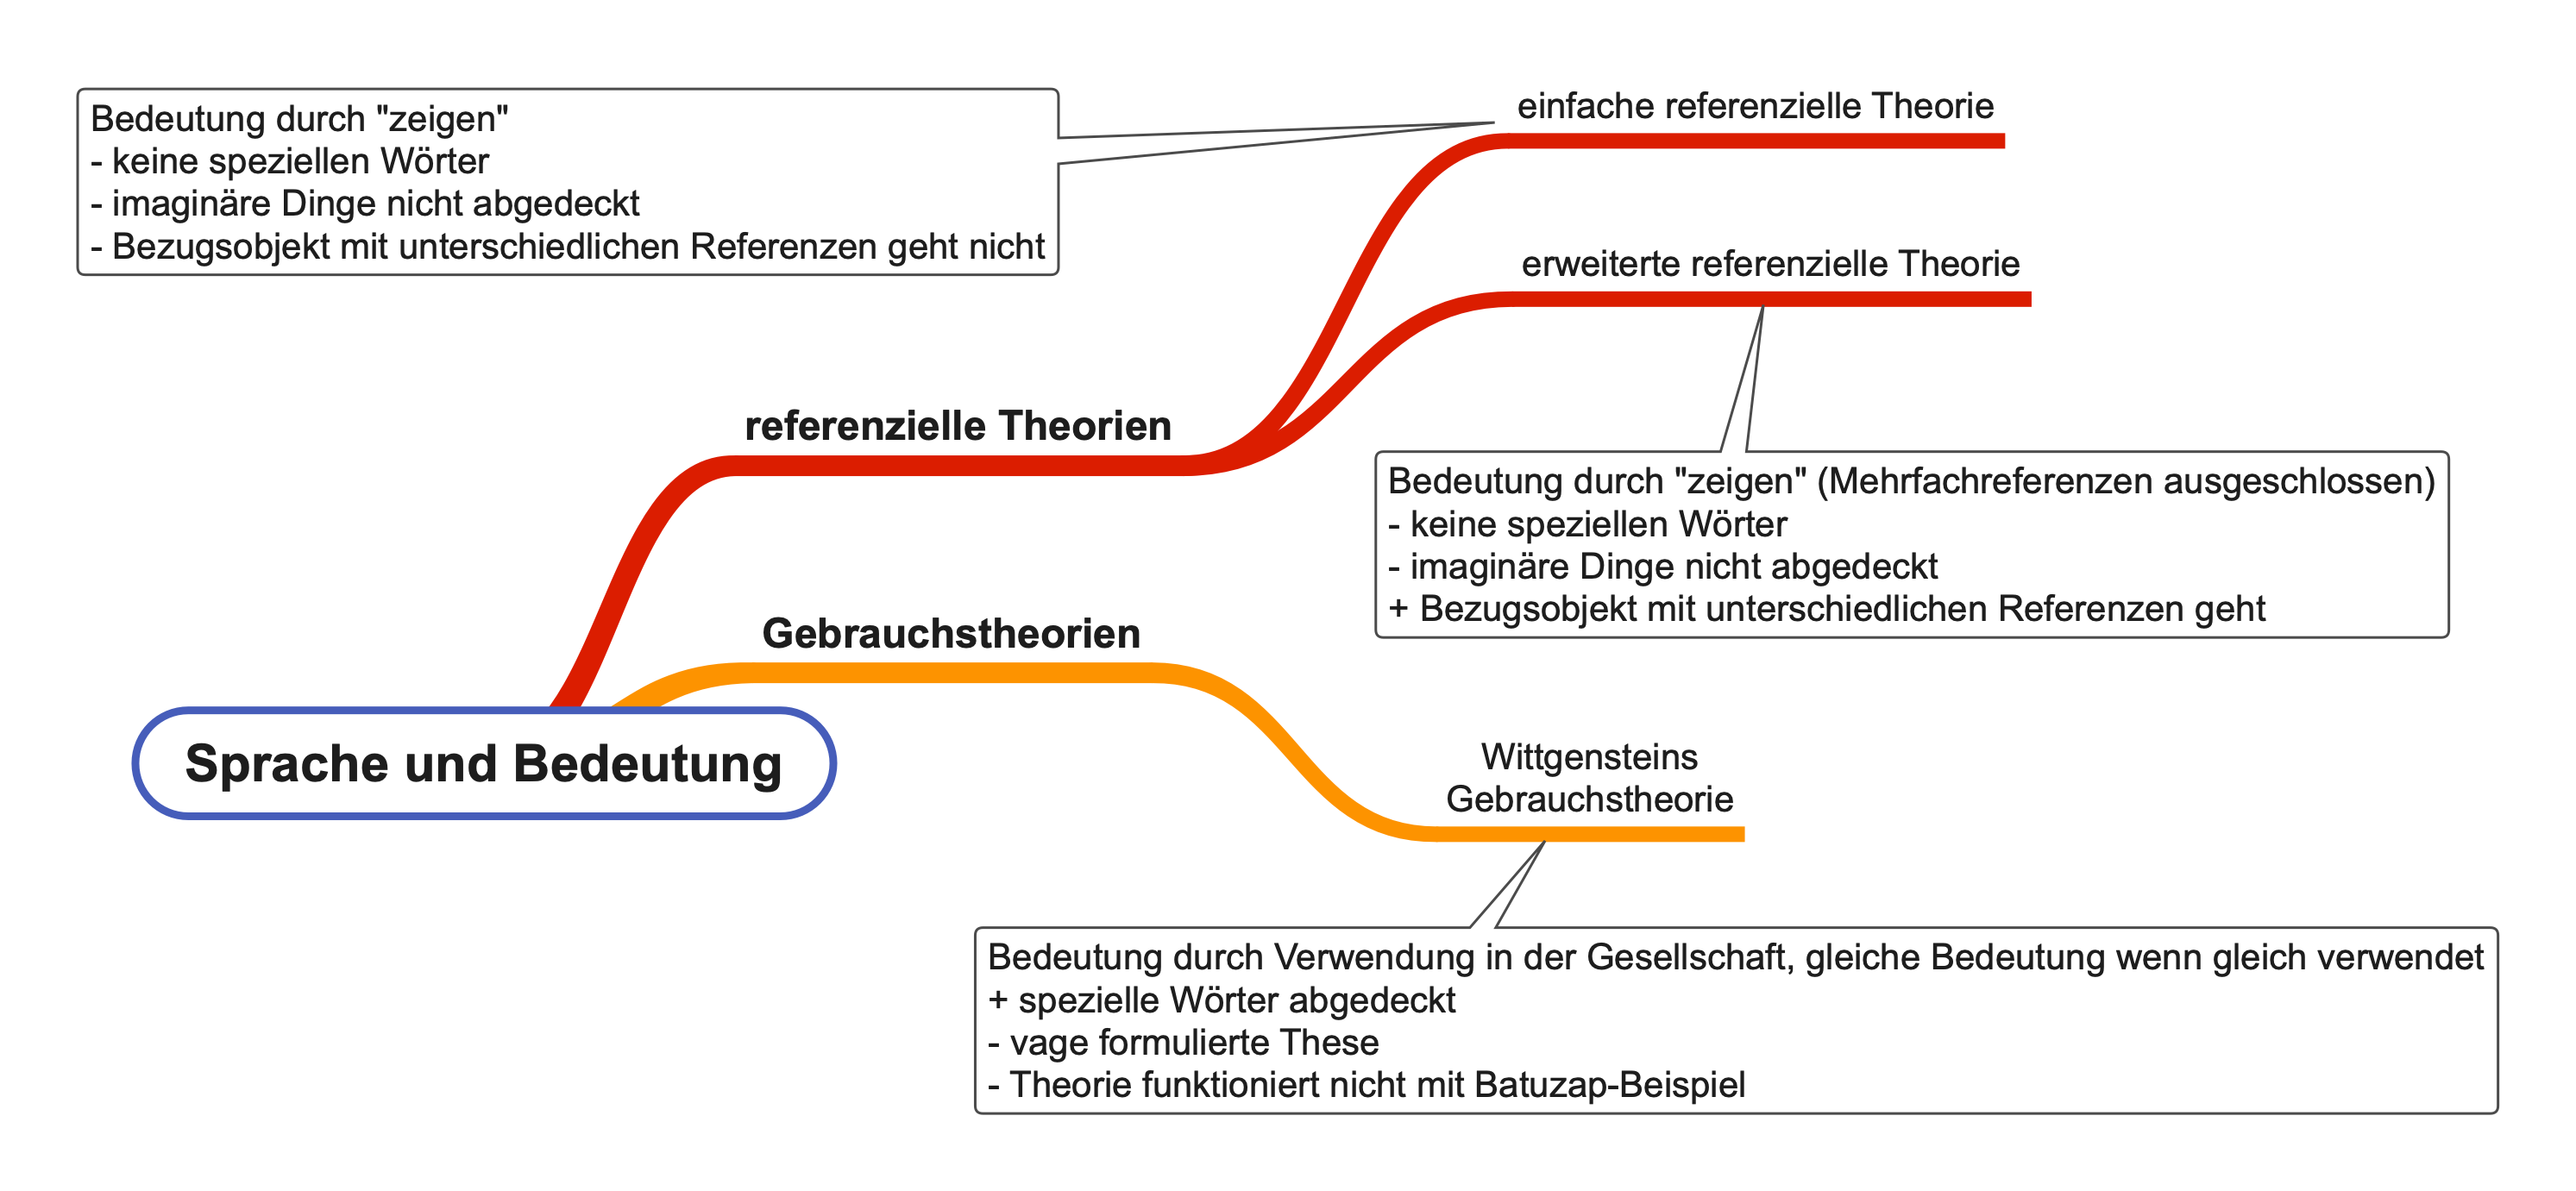
\includegraphics[width=\textwidth]{images/Sprache_und_Bedeutung_Uebersicht.png}

\section{Was ist Sprachphilosophie?}
\paragraph{Problem} Was ist sprachliche Bedeutung und wie erhalten Begriffe eine Bedeutung, resp. wie definiert sich diese? Was ist sprachlicher Bezug (Referenz) und wie lässt sich dieser erklären? Was kann man mit Sprache alles tun? Was heisst es, zu \emph{verstehen}?

\paragraph{Abgrenzung} Die Sprachphilosphie beschäftig sich mit Systemen und Kompetenz der Sprache im Allgemeinen. Z.B. \textit{Was lässt sich alles mit Sprache ausdrücken?} oder \textit{Wie erlangt unsere Sprache Bedeutung?}. Die Sprachphilosophie kümmert sich aber nicht mit Eigenheiten verschiedener Sprachen und ist nicht zu verwechseln mit Linguistischer Philosophie, nach welcher die ganze Philosophie mit Sprache zu tun hat und philosophische Probleme nur auf begrifflichen Unklarheiten beruhen (die sich durch genaue Definitionen auflösen lassen).

\paragraph{Gliederung der Sprachphilosophie} Die Sprachphilosophie gliedert sich in:
\begin{itemize}
  \item Syntax (interne Struktur von Sprache)
  \item Semantik (Beziehung zwischen der Sprache und der Welt)
  \item Pragmatik (Sprache in kommunikativen Kontext)
\end{itemize}

\section{Was heisst <<Bedeutung>>?}

Mit <<Bedeutung>> ist die <<nicht-natürliche Bedeutung>> (Paul Grice) von Sprache gemeint. Also den Bezug zwischen einem sprachlichen Ausdruck und dessen Bezug in der Realität wie z.B. \textit{Das Läuten bedeutet, dass die Vorlesung zu Ende ist.}. Nicht gemeint ist der Ausdruck von Relevanz (\textit{Das bedeutet mir etwas.}) oder <<natürliche Bedeutung>> (\textit{Du hast Krebst, das bedeutet, dass du bald sterben wirst.})

Es gilt zu beachten, dass im Englischen das Verb \textit{to mean} im Deutschen sowohl (im Deutschen) \textit{meinen} wie auch \textit{bedeuten} umfasst. 

\section{Referenzielle Theorien der Bedeutung}
Referenzielle Theorien versuchen die Bedeutung von Sprache alleine mit der Referenz auf ein physisches Objekt zu erklären. 

\subsection{Einfache referenzielle Theorie der Bedeutung (Gegenstandstheorie)}\label{SectionGegenstandstheorie}
\begin{infobox}
Die Gegenstandstheorie erklärt sprachliche Bedeutung durch sprachlichen Bezug, erklärt jedoch nicht, was dafür verantwortlich ist, dass sich ein Ausdruck auf einen Gegenstand bezieht (die Theorie ist unvollständig). Zusätzlich leidet die Theorie an einigen internen Problemen und wird, aufgrund der Einwände, verworfen. Sie reduziert jedoch die beiden Probleme \textit{Bedeutung und Bezug} auf eines, den \textit{Bezug}.	
\end{infobox}

\paragraph{These} Die Bedeutung eines Ausdrucks ist der Gegenstand, auf den er sich bezieht.

\paragraph{Erklärung} Indem (mit dem Finger) auf einen Gegenstand verwiesen wird, wird die Bedeutung des Wortes erklärt. Die macht Sinn, solange man sogenannte <<singuläre Termini>> (Ausdrücke, die sich auf einen einzelnen Gegenstand beziehen) betrachtet. Diese gliedern sich in drei Klassen: \textit{Eigennamen} (die Namen von Personen und Dingen), \textit{Kennzeichnungen} (eindeutige Beschreibungen) und \textit{indexikalische Ausdrücke} (reine wie 'ich' oder 'hier' und demonstrative wie 'dies' oder 'dort').

\paragraph{Probleme} Die Probleme der einfachen Gegenstandstheorie sind vielfältig:
\begin{enumerate}
	\item Schon demonstrative singuläre Termini lassen sich kaum abbilden (Wie will ich mit einfachem Zeigen die Bedeutung von 'dort' erklären?)
	\item Wie können Kategorien von Objekten mit einfachem Zeigen erklärt werden? Hierbei könnte man entgegnen, dass sich, (1) wenn man auf einen schlafenden Menschen verweist, ich auf die Menge aller schlafenden Menschen verweise oder (2) dass ich mich damit auf die Eigenschaft des <<Schlafens>> verweise.
\end{enumerate}

\paragraph{Einwände} Auch die Einwände (Logikfehler) sind vielfältig:
\begin{enumerate}
	\item 
		Die einfache Gegenstandstheorie besagt, dass die Bedeutung von einem Wort gleich dem Gegenstand ist, auf den man zeigt. Doch (gemäss Gilbert Ryle) begeht man damit einen Kategorienfehler, denn <<Andrin ist 174cm gross.>> $\neq$ <<'Andrin' ist 174cm gross>>.

		Es lässt sich jedoch entgegen, dass, obwohl der Bezugsgegenstand nicht mit der Bedeutung des Ausdrucks gleich ist, die Bedeutung des Ausdrucks durch seinen Bezugsgegenstand festgelegt wird. Es lässt sich also die Bedeutung klären, ohne die beiden Dinge gleichzusetzen.
		
		Es ergibt sich dadurch die \textbf{modifizierte Gegenstandstheorie}, nach der (1) ein Ausdruck eine Bedeutung hat, gdw. er sich auf einen Gegenstand bezieht und (2) zwei Ausdrücke haben dieselbe Bedeutung, gdw. sie sich auf denselben Gegenstand beziehen. Somit lässt sich dieser Einwand umgehen.
	
	\item 
		Es gibt Ausdrücke, die offenkundig Bedeutung haben, sich jedoch nicht auf Gegenstände beziehen. Zum Beispiel Quantoren wie <<alle>> oder <<niemand>>, Konjunktoren wie <<und>> oder <<nicht>> oder Präpositionen wie <<mit>> oder <<auf>>. Solche Ausdrücke lassen sich nicht erklären durch die einfache (oder erweiterte) Gegenstandstheorie.
	\item \label{EinwandDerMehrdeutigenBeschreibungGegenstandstheorie}
		Wenn sich mehrere verschiedene Kennzeichnungen auf ein und denselben Gegenstand beziehen aber in ihrer (eindeutig) beschreibenden Bedeutung unterschiedliche sind, müssten die Ausdrücke \textit{analytisch wahr} (die zugeschrieben Prädikaten müssen sich aus dem Begriff des Subjektes ergeben) sein. Das sind sie aber nicht!
		
		Umgekehrt gibt es Ausdrücke wie <<ich>>, die sich kontextabhängig auf verschiedene Dinge beziehen können.
	\item 
		Nimmt man eine wahre Behauptung über die Nicht-Existenz eines imaginären Wesens (Nikolaus), bricht dies die Gegenstandstheorie. Denn ein solches imaginäres Wesen ist nicht verweisbar, demzufolge hat der Satz keine Bedeutung und somit ist der gesamte Ausdruck nicht wahr. Die Gegenstandstheorie kann dies nicht abdecken.
		
		Selbst wenn sich die Bedeutung des Ausdrucks auf eine Vorstellung im Geiste bezieht, funktioniert die Theorie nicht. Denn dann wäre die wahre Behauptung über die Nicht-Existenz ja nicht wahr, sondern falsch (das Wesen existiert in meiner Vorstellung).
\end{enumerate}

\section{Gebrauchstheorien der Bedeutung}
Gebrauchstheorien versuchen die Bedeutung von Sprache mit ihrem Gebrauch (in der Gesellschaft) zu erklären. Begründer ist Ludwig Wittgenstein. Er erkannte, dass, wenn wir das Wort <<Bedeutung>> verwenden, wir eigentlich nicht das Ding bezeichnen, auf das es verweist. 

\subsection{Wittgensteins Gebrauchstheorie der Bedeutung}\label{SectionWittgensteinsGebrauchstheorie}
\paragraph{These}\label{these_gebrauchstheorie} (1) Ein Ausdruck hat Bedeutung, gdw. er (von einer Gemeinschaft) in einer bestimmten Art und Weise verwendet wird und (2) zwei Ausdrücke haben dieselbe Bedeutung gdw. ihre Verwendung (in der Gemeinschaft) in relevanter Hinsicht identisch ist. 

\paragraph{Erklärung} Wir erlernen und erklären Wörter mit ihrem Kontext (wie sie gebraucht werden). Wir wissen, was ein Wort bedeutet, wenn wir wissen, wie es verwendet wird. Für gewisse Ausdrücke können hinweisend (einfache Gegenstandstheorie) erklärt werden, andere (z.B. Quantoren) werden im Zusammenhang erklärt. Somit nimmt die Gebrauchstheorie gewisse Aspekte der Gegenstandstheorie auf, erweitert und uminterpretiert diese jedoch.

\paragraph{Probleme} Die Gebrauchstheorie (\ref{these_gebrauchstheorie}) ist sehr wage formuliert. So stellt sich die Frage, in welcher \textit{bestimmten} Art und Weise Wörter verwendet werden oder in welcher \textit{bestimmten} relevanten Hinsicht zwei Wörter gleichbedeutend sind.

\paragraph{Einwände}
\begin{enumerate}[listparindent=0.7cm]
	\item 
		Nimmt man sinnfreie Ausdrücke wie <<ba>> und <<tu>> und trainiert eine Gruppe von Menschen darauf, diese in einer bestimmten Reihenfolge zu verwenden, haben wir dann bereits Ausdrücke mit Bedeutung geschaffen? Oder anders ausgedrückt: Handelt es sich, gemäss der Gebrauchstheorie, um Ausdrücke?
		
		Man könnte nun sagen, dass dieses Gebilde zu wenig komplex ist, aber selbst mit einem umfangreichen und komplexem Regelsystem werden wir kaum von Zeichen \textit{mit Bedeutung} reden können. 
Auch scheint die beschriebene Verwendungsweise nicht der Art zu entsprechen, die dafür sorgt, dass Ausdrücke eine Bedeutung erhalten (Bezug auf Dinge/Eigenschaften in der Welt). So ist die reale Sprache nicht lediglich ein Mechanismus mit Reihenfolge (auf <<Danke>> einfach folgt <<Bitte>>), sondern ist immer eingebetet im Kontext eines grösseren Ganzen (in Bitte-Danke die Praxis des Gebens und Nehmens). Das Batuzap-Beispiel ähnelt eher einem gesellschaftlichen Tanz.

		Dies ändert sich jedoch, alsbald wir den einfachen Ausdrücken eine reale Bedeutung/Konsequenz zuschreiben. Muss nämlich nach der Nennung einer dieser Ausdrücke eine bestimmte Handlung erfolgen, so haben wir damit reale Kommunikation geschaffen. Denn Sprache (im robusten Sinn) hat etwas mit (1) aussersprachlichen Praktiken zu tun und (2) mit der aussersprachlichen Realität.
	\item 
		Alstons Antwort... % TODO Alstons Antwort 
\end{enumerate}

\end{document}